% 可将两个 figure 分别插入第九部分对应小节；路径相对 Xelatex 主目录。
\begin{figure}[htbp]
 \centering
 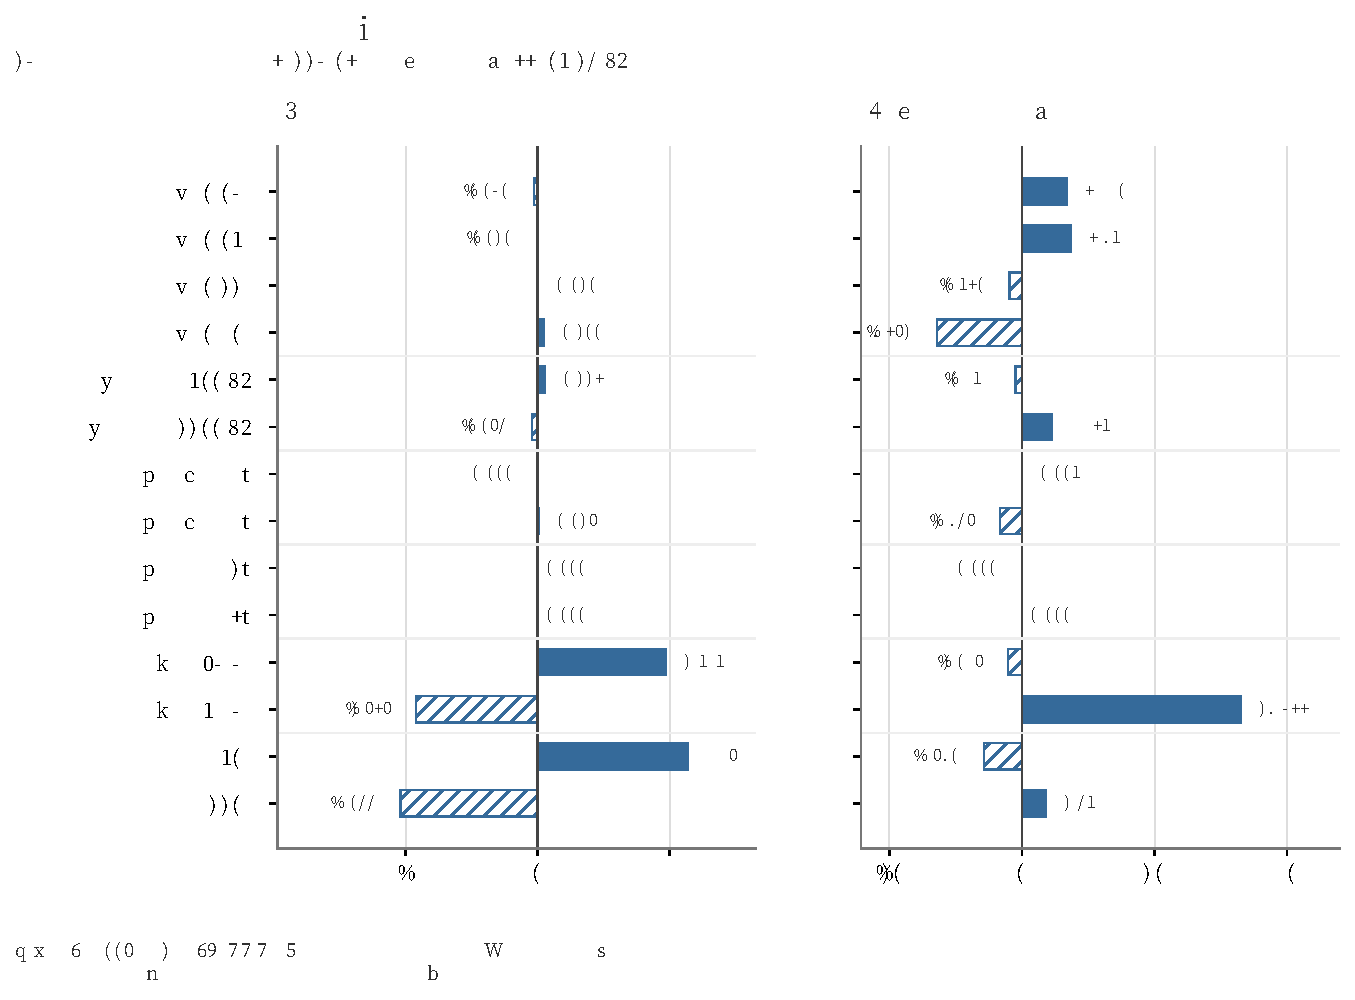
\includegraphics[width=\textwidth]{final_results/section9_visuals/q1_sensitivity.pdf}
 \caption{问题一单参数重求解的敏感性。变化率以基准方案为参照，实心与斜线分别表示增加和减少，两个面板采用不同横轴尺度。}
 \label{fig:section9-q1-sensitivity}
\end{figure}

\begin{figure}[htbp]
 \centering
 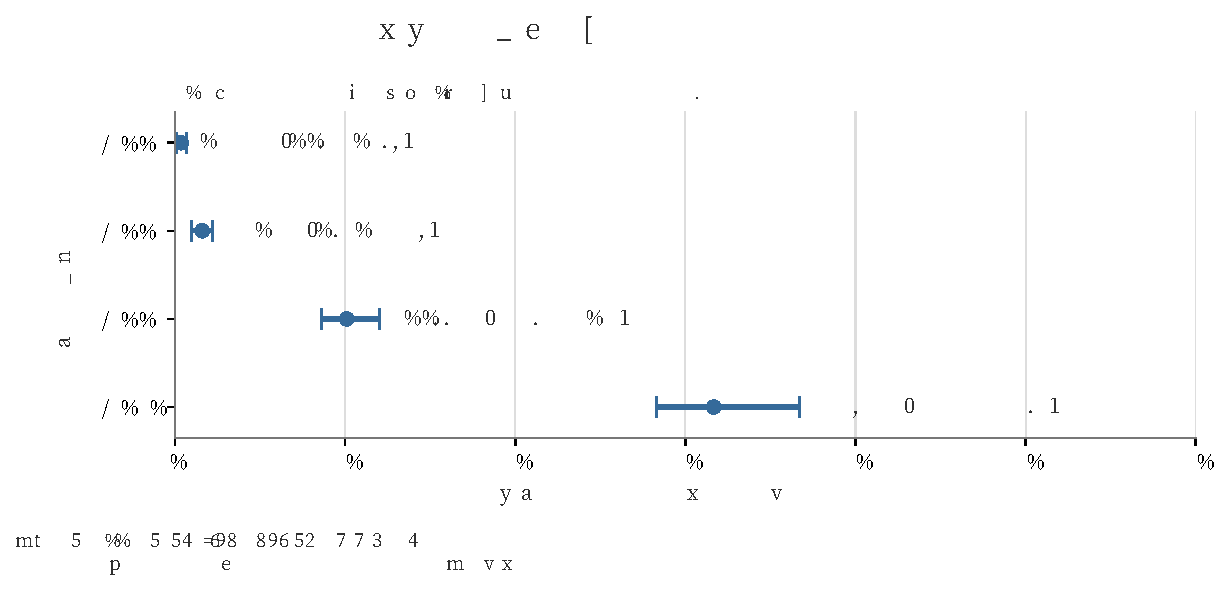
\includegraphics[width=\textwidth]{final_results/section9_visuals/q2_execution_stress.pdf}
 \caption{第二问历史固定计划的相关噪声执行回放。圆点为30次重复的费用平均变化，横线为5\%至95\%经验分位；该区间不表示未来实际费用的置信区间。}
 \label{fig:section9-q2-stress}
\end{figure}
